\documentclass[letterpaper,twocolumn,amsmath,amssymb,pre,aps,10pt]{revtex4-1}

\usepackage{graphicx}% Include figure files
\usepackage{color}

\newcommand{\fixme}[1]{{\bf\color{red}{[#1]}}}
\newcommand{\rr}{\mathbf{r}}

\begin{document}
\title{Renormalization}

\author{Daniel E. Roth}
\author{Michael ?. Perlin}
\author{David Roundy}
\affiliation{Department of Physics, Oregon State University, Corvallis, OR 97331}

\begin{abstract}
  We present an analysis of the convergence properties of
  renormalization group theory  when applied to the square-well
  liquid.
\end{abstract}

\maketitle

Long-wavelength fluctuations lead to significant changes in fluid
behavior in two scenarios: near the critical point, and at
liquid-vapor interfaces.  The failing of perturbation theory near the
critical point is well-understood, and is commonly treated in the
homogeneous case using either renormalization group
theory~\cite{white2000global, white2001global, del2002vapour,
  kiselev2002computer, reiner2002hierarchical, mi2004renormalization,
  mi2004improved, fu2006study, giacometti2009liquid, jiuxun2005simple,
  forte2011application, el2008integral, ramana2012generalized}, or
crossover theory~\cite{kiselev1999crossover, kiselev2000crossover,
  kiselev2001crossover, kiselev2000simplified, hu2003crossover,
  hu2003back, mccabe2004crossover, llovell2006global}.  The
liquid-vapor interface is beset by long-wavelength fluctuations in the
form of capillary waves~\cite{buff1965interfacial,
  weeks1989consistency}, which are handled---when treated at all---as
an analytic correction to the surface tension computed using density
functional theory~\cite{wadewitz2000application, winkelmann2001liquid,
  gross2009density}.  These corrections to the surface tension involve
an ad hoc cutoff wavelength, and do not correct the prediction of the
interfacial density profile.  The effect of capillary waves on surface
tension is largest near the critical point.  Together, these effects
suggest that a density functional theory directly incorporating
long-wavelength fluctuations would be a major gain for the study of
liquid interfaces.

I plan to develop such a functional using renormalization group theory
(RGT).  Implementation of RGT in an inhomogeneous system will be
computationally challenging, because it is an inherently recursive
theory.  This results in long-range fluctuations (and correlations)
near the critical point, which will be reflected in a long-range
density functional.  It will be more computationally
intensive than existing density functionals, but at the same time will
enable far greater predictive power, over a wide range of
temperatures, pressures, and density distributions.

There has been one study of the effect of critical behavior on surface
tension using a renormalization approach, which used the Density
Gradient Theory (DGT) rather than DFT due to its easier integration
with renormalization group theory~\cite{fu2006study}.  The use of DGT,
which is not self-consistent, puts a major limitation the power of the
method, particularly when applied to diverse interfaces.


We will study a hard-sphere fluid with a square well attractive
potential.  This is a widely used model fluid within the SAFT
community~\cite{mi2004renormalization, mi2004improved, fu2006study,
  forte2011application} as well as in the study of the critical
behavior of fluids~\cite{white2000global, white2001global,
  del2002vapour, kiselev2002computer, reiner2002hierarchical,
  mi2004renormalization, mi2004improved, fu2006study,
  giacometti2009liquid, jiuxun2005simple, forte2011application,
  el2008integral, ramana2012generalized}. This model is particularly
suitable for testing over a wide range of temperatures and pressures
due to its ease of computation.  Because the set of energy levels is
discrete, this system is suitable for the use of histogram-based Monte
Carlo methods~\cite{ferrenberg1988histogram, lee1993new, de1998broad}.
These approaches accelerate the computation of thermodynamic
properties over a range of temperatures, and are particularly helpful
near phase transitions and critical points.  There has been a recent
Monte Carlo study of phase behavior of the the square-well
fluid~\cite{liu2005direct}, which did not take advantage of the
histogram family of Monte Carlo methods, although it did use the
aggregation volume bias sampling method to accelerate sampling of
bonded and non-bonded configurations~\cite{chen2000novel}.

We will begin by studying the simple square-well liquid already
introduced in a previous paragraph.  This liquid is a standard test
case for theories of critical behavior, although its critical behavior
at the liquid-vapor interface has not yet been examined.  We will
closely follow the approach recently developed by Forte \emph{et al.}
who constructed a SAFT-VR equation of state using
RGT~\cite{forte2011application}.  Their approach to RGT is expressed
in terms of the pair distribution function
$g^{(2)}_{HS}(\rr_1,\rr_2)$, which will enable us to leverage our
earlier work (from the previous paragraph) to construct a
renormalization group classical density functional theory for the
inhomogeneous fluid.  Once we have developed a RGT density functional,
we will test it against Monte Carlo simulations of the surface
tension, as well as a fluid near the critical point at a hard wall.
%
Future work will include applying this approach to associating fluids.


\section{Methods}

\subsection{Renormalization Group Theory}

\begin{figure}
  \centering
  \includegraphics[width=0.8\columnwidth]{figs/RG_comparison}
  \caption{Grand free energy per unit volume for different iteration depths}
\end{figure}

\subsubsection{Defining our approximation}
Let's begin by considering the partition function and free energy, as
computed in the canonical ensemble:
\begin{align}
  Z &= \sum_i^{\text{\tiny\begin{minipage}{5em}
      \begin{center}
        \tiny all microstates\end{center}\end{minipage}}}
       e^{-\beta E_i}, & F &= -kT\log Z
\end{align}
We now consider a ``smooth'' configuration that contains only
microstates that are periodic with a given periodicity $2^j\lambda$:
\newcommand\sumstatesperiodic[1]{\sum_i^{\text{\tiny\begin{minipage}{6em}
      \begin{center}
        \tiny microstates periodic $#1$\end{center}\end{minipage}}}}
\begin{align}
  Z_j &= \sumstatesperiodic{2^j\lambda}
       e^{-\beta E_i}, & F_j &= -kT\log Z_j
       \label{eq:Zn}
\end{align}
This defines a family of free energies that contain fluctuations with
a variety of length scales.  For the moment we will assume a simple
cubic periodicity, although it may be advantageous to select face
centered cubic (FCC) instead.  So far, we have defined a family of
free energy functions (each containing longer length-scale
fluctuations) that we can compute numerically using Monte Carlo, but
we have not yet constructed a means to approximate these functions.
Before developing this approximation, let's reorganize this sum over
periodic states.
\begin{figure}
  \centering
  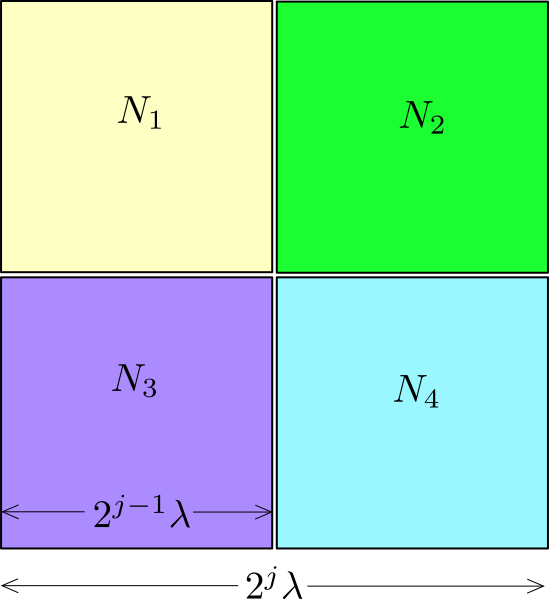
\includegraphics[width=0.8\columnwidth]{figs/divisions}
  \caption{A cell being subdivided with $N_1\cdots N_8$ particles in
    each subdivision.}
\end{figure}
\newcommand\sumoccupanciesofoctants{
  \sum_{N_1\cdots N_8}^{\text{\tiny\begin{minipage}{5em}
      \begin{center}
      \tiny numbers in octants\end{center}\end{minipage}}}
}
\newcommand\summicrostatesofoctants{
  \sum_{i_1\cdots i_8}^{\text{\tiny\begin{minipage}{4em}
      \begin{center}
      \tiny microstates\\within octants\end{center}\end{minipage}}}
}
\begin{align}
  Z_j(N) &= \sumoccupanciesofoctants g_{N_1\cdots N_8}
       \summicrostatesofoctants
       e^{-\beta E_{i_1\cdots i_8}^{(j)}}
\end{align}
where here $g_{N_1\cdots N_8}$ is a multiplicity factor
corresponding to the number of ways the cell can be divided into
subcells with occupancies of $N_1\cdots N_8$.  This is so far only a
different way of writing Eq.~\ref{eq:Zn}.  At this point, we can
multiply and divide by a few factors, with a goal of replacing the
unknown $E_{i_1\cdots i_8}^{(j)}$ with something that is easier to
approximate.
\begin{multline}
  F_j(n) = -kT\log\Bigg(
    \sumoccupanciesofoctants
       g_{N_1\cdots N_8}
       \\
       \summicrostatesofoctants
       e^{-\beta E_{i_1\cdots i_8}^{(j)}}
  \Bigg)
\end{multline}

\subsubsection{Free energy of the sub-systems}

Now we consider the same free energy computed without accounting for
the energy in the fluctuations:
\begin{multline}
  F_{j-1}(n) = -kT\log\Bigg(
    \sumoccupanciesofoctants
       g_{N_1\cdots N_8}
       \\
       \summicrostatesofoctants
       e^{-\beta \left(E_{i_1}^{(j-1)} + \cdots + E_{i_8}^{(j-1)}\right)}
  \Bigg)\label{eq:Fjm1}
\end{multline}
We can now recognize that each of the octants is just a similar smooth
system.

The multiplicity term $g_{N_1\cdots N_8}$ that shows up in
Eq.~\ref{eq:Fjm1} (and elsewhere) originates from the choice made when
splitting our sum over all microstates into separate sums for
microstates in each of the octants.  This required us to pick a
combination of states for each octant, thus the $g_{N_1\cdots N_8}$.
This multiplicity is given by:
\begin{align}
  g_{N_1\cdots N_8} &=
  {N \choose N_1} {N - N_1 \choose N_2} {N - N_1 - N_2 \choose N_3}
  \cdots \\
  &\propto \sum_{i=1}^{8} N_i!
  \\
  &\approx \sum_{i=1}^{8} (N_i-1) e^{N_i}
\end{align}
Physically, this multiplicity term corresponds to the ideal gas
contribution to the free energy.  In fact, the ideal gas free energy
represents \emph{only} the multiplicity and kinetic energy.  Since the
free energy incorporates the multiplicity, we can simplify
Eq.~\ref{eq:Fjm1} as:
\begin{multline}
  F_{j-1}(n) = -kT\log\Bigg(
    \sumoccupanciesofoctants
       e^{-\beta \left( F_{j-1}(N_1) + \cdots F_{j-1}(N_8) \right)}
  \Bigg)
\end{multline}
where I have introduced the confusing notation where $F_{j-1}(n)$
represents the free energy computed for any density $n$ representable
in the $2^j\lambda$ cell by averaging over particle distributions
$N_1\cdots N_8$, while $F_{j-1}(N)$ represents the canonical free
energy found for a set of microstates with $N$ particles in the cell
volume.

Putting these last two equations together, we can find a formula for
the energy difference as we include the larger fluctuations:
\begin{multline}
  F_j(n) - F_{j-1}(n) =\\
  -kT\log\left(\frac{
    \sumoccupanciesofoctants
       g_{N_1\cdots N_8}
       \summicrostatesofoctants
       e^{-\beta E_{i_1\cdots i_8}^{(j)}}
  }{
    \sumoccupanciesofoctants
        e^{-\beta \left( F_{j-1}(N_1) + \cdots F_{j-1}(N_8) \right)}
  }
  \right)
\end{multline}
At this point, we recognize that we can put anything we like in the
numerator \emph{and} the denominator, which will help us to prevent
the exponentials from getting too hairy.  This is really just a shift
of energy for both the numerator and denominator partition functions.
\begin{multline}
  F_j(n) - F_{j-1}(n) =\\
  -kT\log\left(\frac{
    \sumoccupanciesofoctants
       g_{N_1\cdots N_8}
       \summicrostatesofoctants
       e^{-\beta \left(E_{i_1\cdots i_8}^{(j)}  - F_{j-1}(n) \right)}
  }{
    \sumoccupanciesofoctants
       e^{-\beta \left( F_{j-1}(N_1) + \cdots F_{j-1}(N_8)  - F_{j-1}(n) \right)}
  }
  \right)
\end{multline}
At this stage we have still not introduced an uncontrolled
approximation.  Each $F_{j}$ is exactly defined, and the exact free
energy is found by taking a limit $j\rightarrow \infty$.  \fixme{I
  need to clarify the scale of each $F$.  Some of the above are about
  systems $\frac18$ the volume of others.}

The flavor of the approximation used by White and others in GRG is now
clarified.  We begin by assuming that we already have an adequate (and
tractable) approximation for $F_{j-1}$.  Thus the denominator
partition function is readily computable.  We further simplify the
numerator by multiplying and dividing by the same quantity, and
simplify the notation by defining
\begin{align}
  F_j(N_1\cdots N_8) &= g_{N_1\cdots N_8}
       \summicrostatesofoctants
       e^{-\beta E_{i_1\cdots i_8}^{(j)}}
\end{align}
\begin{widetext}
and thus rewrite the energy difference as
\begin{multline}
  F_j(n) - F_{j-1}(n) =\\
  -kT\log\left(\frac{
    \sumoccupanciesofoctants
       e^{-\beta \big(F_{j-1}(N_1) + \cdots F_{j-1}(N_8)  - F_{j-1}(n) +
           \big(F_j(N_1\cdots N_8) - F_{j-1}(N_1) - \cdots - F_{j-1}(N_8)\big) \big)}
  }{
    \sumoccupanciesofoctants
       e^{-\beta \left( F_{j-1}(N_1) + \cdots F_{j-1}(N_8)  - F_{j-1}(n) \right)}
  }
  \right)
\end{multline}
\end{widetext}
At this point we can recognize and identify two energy differences as
\begin{align}
  \bar{F}(N_1\cdots N_8) &= F_{j-1}(N_1) + \cdots F_{j-1}(N_8)  - F_{j-1}(n) \\
  \bar{U}(N_1\cdots N_8) &= F_j(N_1\cdots N_8)
  - \left(F_{j-1}(N_1) + \cdots + F_{j-1}(N_8) \right)
\end{align}
and using these definitions can rewrite our energy difference in a
more compact form:
\begin{multline}
  F_j(n) - F_{j-1}(n) =\\
  -kT\log\left(\frac{
    \sumoccupanciesofoctants
       e^{-\beta \big( \bar{F}(N_1\cdots N_8) + \bar{U}(N_1\cdots N_8)
         \big)}
  }{
    \sumoccupanciesofoctants
       e^{-\beta \bar{F}(N_1\cdots N_8)}
  }
  \right)
\end{multline}
At this point, we can recognize $\bar{F}(N_1\cdots N_8)$ as the free
energy change due to oscillations \emph{if we neglect the actual
  energy of the oscillations themselves, but instead make a ``local''
  approximation}.  Meanwhile $\bar{U}(N_1\cdots N_8)$ is the free
energy change due to the energy of oscillations.

\begin{figure}
  \centering
  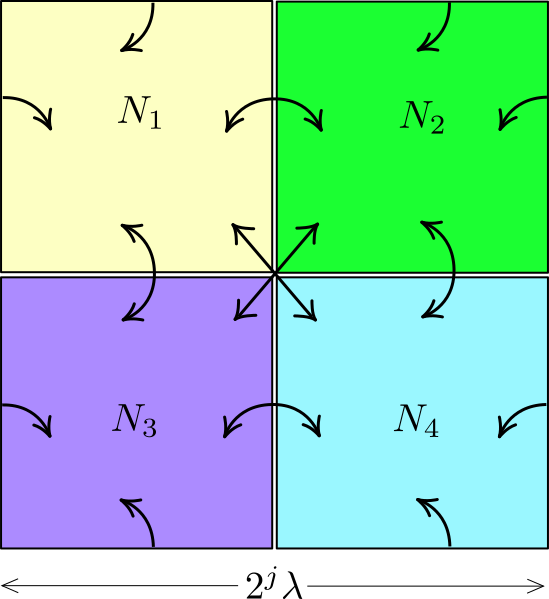
\includegraphics[width=0.8\columnwidth]{figs/interactions}
  \caption{Interactions between all subdivisions.}\label{fig:interactions}
\end{figure}

\subsubsection{Interaction between subsystems}
At this stage, there is just one term that need be approximated
(assuming, as always, that we have an acceptable approximation for
$F_{j-1}$), which is $\bar{U}$.  This is the free energy difference
between two free energies.  The first, $F_j(N_1\cdots N_8)$, is the
fully interacting system that is periodic with periodicity
$2^j\lambda$, and which is constrained to have $N_1\cdots N_8$
particles in each of the subdivisions of the cell.  The second is the
sum of $F_{j-1}$ for each of those subdivisions.  This difference
describes the interaction between the octants of the cell, and is at
the heart of the GRG method.

We desire to simplify the summation over seven independent numbers
$N_1\cdots N_7$ (with the eighth constrained by $\sum_i N_i = N$) to a
summation over a single fluctuation amplitude.  As illustrated in
Fig.~\ref{fig:interactions}, these interactions can be seen as a sum
of interactions between neighboring subdivisions, combined with a
many-body corrections due to the free energy not being precisely
separable into additive pairwise contributions (due to for instance
``corner'' interactions).

\begin{figure}
  \centering
  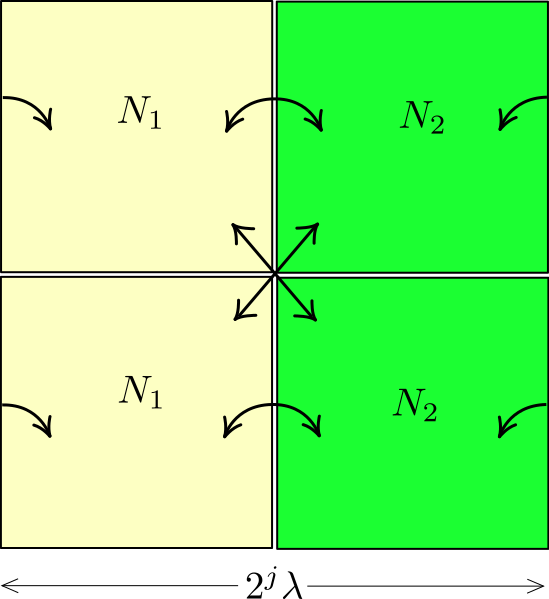
\includegraphics[width=0.8\columnwidth]{figs/neighbors}
  \caption{Interactions between only neighboring subdivisions.}\label{fig:neighbors}
\end{figure}

If we make this assumption, that the free energy can be separated into
neighboring contributions, we can write
\begin{align}
  F_j(N_1\cdots N_8) &= \alpha \sum_{ij}^{\text{neighbors}} F_j^{\text{neighbor}}(N_i, N_j)
\end{align}
where $F_j^{\text{neighbor}}(N_i, N_j)$ is the free energy of the
system illustrated in Fig.~\ref{fig:neighbors}, which has a slab-like
density oscillation, and $\alpha$ \fixme{is a prefactor that I need to
  work out}.

I will note that we have a choice of lattice when defining our
periodic system.  At this point we can see that a simple cubic lattice
gives us a flat-slab neighbor system.  If we had chosen a close-packed
FCC lattice, then each subdivision would interact equally with all the
other subdivisions (and corners would involve four subdivisions rather
than all eight), but our slab geometry would have a bumpy interface
(e.g. if we chose a $\langle 111\rangle$ slab it would have an
equilateral triangular lattice of bumps).  I will continue thinking in
terms of a simple cubic interface, with the option to revise this to
switch lattices.

Once we have rewritten $F_j(N_1\cdots N_8)$ in terms of
$F_j^{\text{neighbor}}(N_i, N_j)$, we can further simplify our free energy
difference (and definitions of $\bar{U}$ and $\bar{F}$):
\begin{multline}
  \sumoccupanciesofoctants
  e^{-\beta \big( \bar{F}(N_1\cdots N_8) + \bar{U}(N_1\cdots N_8)
         \big)}
  \\=
  \sumoccupanciesofoctants
  e^{-\beta \big( F_j(N_1\cdots N_8) - \sum\cdots
         \big)}
  \\\approx
  \sumoccupanciesofoctants
  e^{-\beta \big( F_j^{\text{NN}}(N_1, N_2) + F_j^{\text{NN}}(N_1,
    N_3) + \cdots - \cdots
         \big)}
\end{multline}
Sadly, this does not immediately separate into terms similar to those
in standard GRG.


\subsection{To do later}

\begin{enumerate}
\item \fixme{Elaborate on the approximation (ignoring corners) that
  leads from a $\sumoccupanciesofoctants g_{N_1\cdots N_8}$ to an
  integral over density amplitudes.}
\item \fixme{Develop an approach for approximating $\bar{U}$.  Perhaps
  is $F_{j-1}$ is expressed as a functional, we can use a non-local
  DFT to approximate $\bar U_j$?  The standard GRG approach seems to
  be to use a simple mean-field or thermodynamic perturbation theory
  approach to approximate $\bar U$, suggesting that a simple
  (standard) DFT might work just fine for this.}
\end{enumerate}

\begin{figure}
  \centering
  \includegraphics[width=\columnwidth]{figs/fluctuations}
  \caption{Fluctuations at all length scales}
  \label{fig:fluctuations}
\end{figure}


\subsection{Monte Carlo}

\fixme{Here we will explain our Monte Carlo simulations.}

\section{Results}

\section{Conclusion}

\bibliography{paper}% Produces the bibliography via BibTeX.

\end{document}
